\documentclass{article}




\usepackage{fullpage}
%\usepackage{nopageno}
\usepackage{amsmath}
\usepackage{amsfonts}
\usepackage{graphicx}
\usepackage{framed}
\usepackage{algorithmic}
\usepackage{xcolor}

\definecolor{dark_red}{rgb}{0.5,0.0,0.0}
\definecolor{dark_green}{rgb}{0.0,0.5,0.0}
\definecolor{dark_blue}{rgb}{0.0,0.0,0.5}
\definecolor{blue}{rgb}{0.0,0.0,1.0}

\newcommand{\dr}[1]{\textcolor{dark_red}{#1}}
\newcommand{\dg}[1]{\textcolor{dark_green}{#1}}
\newcommand{\db}[1]{\textcolor{dark_blue}{#1}}
\newcommand{\blue}[1]{\textcolor{blue}{#1}}


\title{MATH2860 - 01 Project \#2}
\date{Summer 2021}

\begin{document}

\maketitle

\begin{center}
\begin{tabular}{cc}
\parbox{0.5\textwidth}{
This project will involve the analysis of elastic meshes. Given a system of elastic beams connected by rigid joints, the deformation of such structures under known forces will be analyzed. 
} & \parbox{0.5\textwidth}{
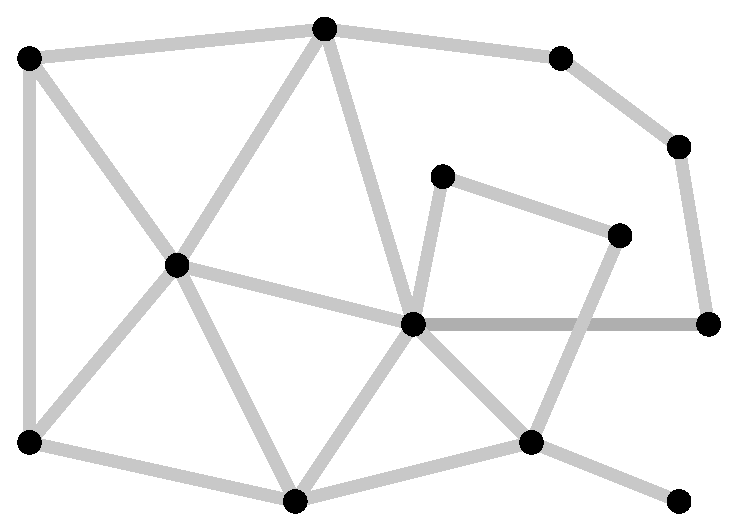
\includegraphics[width = 0.5\textwidth]{elastic_mesh_example}
}
\end{tabular}
\end{center}



\section{Terminology}

The mathematical model used in this project will use the following terminology:

\begin{description}
\item[node] A ``node" is a junction between 1 or more elastic beams. There are two types of nodes: anchored nodes and free floating nodes.
\item[anchored node] An ``anchored node", also referred to as a ``grounded node" borrowing terminology from electrical circuits, is node whose position is fixed.
\item[floating node] A ``floating node" is a node whose position can change as the connecting beams deform under stress. 
\item[bream] A ``beam" is an elastic rod that connects two floating nodes, or a floating node with an anchored node. If one the nodes is anchored, then the beam is referred to as an ``anchored beam". In this mathematical model, the beams will be subject to tension, compression, and shear. Rotation will not be considered as the model will be ``linear". If rotation were to be considered, the system would not be described by a linear system of equations. Beams will also be rotationally symmetric.
\item[stress] ``Stress" is a measure of the forces acting on a structure that cause it to deform.    
\item[strain] ``Strain" is a measure of the deformation a structure undergoes when subjected to stress.
\end{description}

\begin{center}
\begin{tabular}{cc}
\parbox{0.5\textwidth}{
The most important aspect of the mathematical model that is being used for this project is that the model is linear. Linear systems can be described by a system of linear equations, and are considerably easier to solve both analytically and computationally than other ``non-linear" models. To keep the model linear, the beams will be allowed to undergo tension, compression, and shear, but not rotation. The absence of rotation makes the model inaccurate when the deformation (strain) becomes large, but with small deformations, the model is largely accurate. 
} & \parbox{0.5\textwidth}{
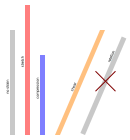
\includegraphics[width = 0.5\textwidth]{tension_compression_shear_no_rotation}
}
\end{tabular}
\end{center}



\section{Setting up the Linear System}

Consider a beam that connects nodes \(i\) and \(j\). Let \(\mathbf{q}_i\) denote the rest coordinate of node \(i\), and \(\mathbf{q}_j\) denote the rest coordinate of node \(j\). 

Let \(\Delta\mathbf{q}_i\) denote the displacement of node \(i\) from its rest point of \(\mathbf{q}_i\), and let \(\Delta\mathbf{q}_j\) denote the displacement of node \(j\) from its rest point of \(\mathbf{q}_j\). Let \(\mathbf{q}_{i,j}\) denote the displacement 

\begin{center}
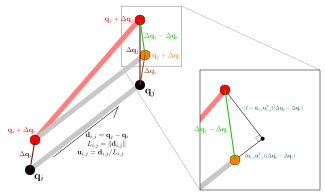
\includegraphics[width = \textwidth]{elastic_beam}
\end{center}



% \frac{t_{g1,1}}{L_{g1,1}}(k_{\text{par}}(\mathbf{u}_{g1,1}\mathbf{u}_{g1,1}^T) + k_{\text{perp}}(I - \mathbf{u}_{g1,1}\mathbf{u}_{g1,1}^T))

\section{Examples}

\begin{tabular}{cc}  
\parbox{0.5\textwidth}{
\[\begin{bmatrix} 
\mathbf{K}_{g1,1}
\end{bmatrix}\begin{bmatrix} 
\Delta\mathbf{q}_1
\end{bmatrix} = \begin{bmatrix}
\mathbf{F}_1
\end{bmatrix}\]
} & \parbox{0.5\textwidth}{
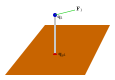
\includegraphics[width = 0.5\textwidth]{elastic_mesh_example_1}
}
\end{tabular}




\begin{tabular}{cc}  
\parbox{0.5\textwidth}{
\[\begin{bmatrix} 
\mathbf{K}_{g1,1} + \mathbf{K}_{g2,1}
\end{bmatrix}\begin{bmatrix} 
\Delta\mathbf{q}_1
\end{bmatrix} = \begin{bmatrix}
\mathbf{F}_1
\end{bmatrix}\]
} & \parbox{0.5\textwidth}{
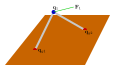
\includegraphics[width = 0.5\textwidth]{elastic_mesh_example_2}
}
\end{tabular}




\begin{tabular}{cc}  
\parbox{0.5\textwidth}{
\[\begin{bmatrix} 
\mathbf{K}_{g1,1} + \mathbf{K}_{1,2} & -\mathbf{K}_{1,2} \\ 
-\mathbf{K}_{1,2} & \mathbf{K}_{1,2}
\end{bmatrix}\begin{bmatrix} 
\Delta\mathbf{q}_1 \\ 
\Delta\mathbf{q}_2
\end{bmatrix} = \begin{bmatrix}
\mathbf{0} \\ 
\mathbf{F}_2 
\end{bmatrix}\]
} & \parbox{0.5\textwidth}{
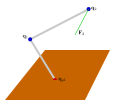
\includegraphics[width = 0.5\textwidth]{elastic_mesh_example_3}
}
\end{tabular}





\[\begin{bmatrix} 
\mathbf{K}_{g1,1} + \mathbf{K}_{1,2} + \mathbf{K}_{1,3} & -\mathbf{K}_{1,2} & -\mathbf{K}_{1,3} \\ 
-\mathbf{K}_{1,2} & \mathbf{K}_{g2,2} + \mathbf{K}_{1,2} & \mathbf{0} \\  
-\mathbf{K}_{1,3} & \mathbf{0} & \mathbf{K}_{1,3}
\end{bmatrix}\begin{bmatrix} 
\Delta\mathbf{q}_1 \\ 
\Delta\mathbf{q}_2 \\ 
\Delta\mathbf{q}_3
\end{bmatrix} = \begin{bmatrix}
\mathbf{0} \\ 
\mathbf{0} \\ 
\mathbf{F}_3 
\end{bmatrix}\]

\begin{center}
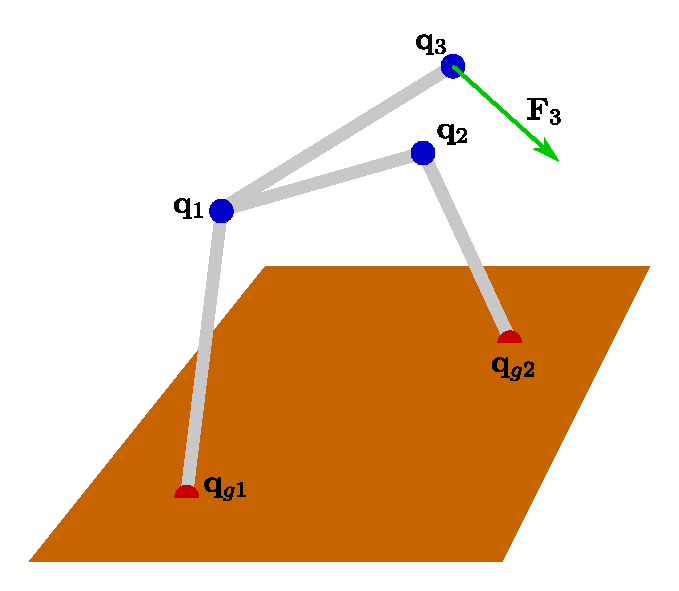
\includegraphics[width = 0.5\textwidth]{elastic_mesh_example_4}
\end{center}




\[\begin{bmatrix} 
\mathbf{K}_{g1,1} + \mathbf{K}_{1,2} + \mathbf{K}_{1,4} & -\mathbf{K}_{1,2} & \mathbf{0} & -\mathbf{K}_{1,4} \\ 
-\mathbf{K}_{1,2} & \mathbf{K}_{g2,2} + \mathbf{K}_{1,2} + \mathbf{K}_{2,3} & -\mathbf{K}_{2,3} & \mathbf{0} \\
\mathbf{0} & -\mathbf{K}_{2,3} & \mathbf{K}_{g3,3} + \mathbf{K}_{2,3} + \mathbf{K}_{3,4} & -\mathbf{K}_{3,4} \\ 
-\mathbf{K}_{1,4} & \mathbf{0} & -\mathbf{K}_{3,4} & \mathbf{K}_{g4,4} + \mathbf{K}_{1,4} + \mathbf{K}_{3,4}
\end{bmatrix}\begin{bmatrix} 
\Delta\mathbf{q}_1 \\ 
\Delta\mathbf{q}_2 \\
\Delta\mathbf{q}_3 \\ 
\Delta\mathbf{q}_4
\end{bmatrix} = \begin{bmatrix}
\mathbf{F}_1 \\
\mathbf{0} \\ 
\mathbf{F}_3 \\ 
\mathbf{0} 
\end{bmatrix}\]

\begin{center}
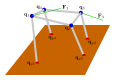
\includegraphics[width = 0.5\textwidth]{elastic_mesh_example_5}
\end{center}




\section{Assignment}

%\begin{itemize}
%\item \texttt{num\_of\_g\_nodes}
%\item \texttt{num\_of\_nodes}
%\item \texttt{g\_node\_coordinates}
%\item \texttt{node\_coordinates}
%\item \texttt{num\_of\_g\_beams} 
%\item \texttt{num\_of\_beams}
%\item \texttt{g\_beam\_end\_nodes}
%\item \texttt{beam\_end\_nodes}
%\item \texttt{g\_beam\_thicknesses}
%\item \texttt{beam\_thicknesses}
%\item \texttt{g\_beam\_stiffnesses}
%\item \texttt{beam\_stiffnesses}
%\item \texttt{g\_beam\_breaking\_limits}
%\item \texttt{beam\_breaking\_limits}
%\item \texttt{forces}
%\end{itemize}

\begin{itemize}
\item \texttt{num\_of\_g\_nodes}
\item \texttt{num\_of\_nodes}
\item \texttt{g\_nodes}
	\begin{itemize}
	\item \texttt{name}
	\item \texttt{x}
	\item \texttt{y}
	\item \texttt{z}
	\end{itemize}
\item \texttt{nodes}
	\begin{itemize}
	\item \texttt{name}
	\item \texttt{x}
	\item \texttt{y}
	\item \texttt{z}
	\item \texttt{F\_x} 
	\item \texttt{F\_y} 
	\item \texttt{F\_z} 
	\end{itemize}
\item \texttt{num\_of\_beams}
\item \texttt{beams}
	\begin{itemize}
	\item \texttt{start}
	\item \texttt{end}
	\item \texttt{t} 
	\item \texttt{k\_par} 
	\item \texttt{k\_perp}
	\item \texttt{ka\_par} 
	\item \texttt{ka\_perp}
	\item \texttt{break\_par}
	\item \texttt{break\_perp}
	\end{itemize}
\end{itemize}




\end{document}


